\chapter{Asociación Calificada}
\begin{figure}[h]
	\centering
	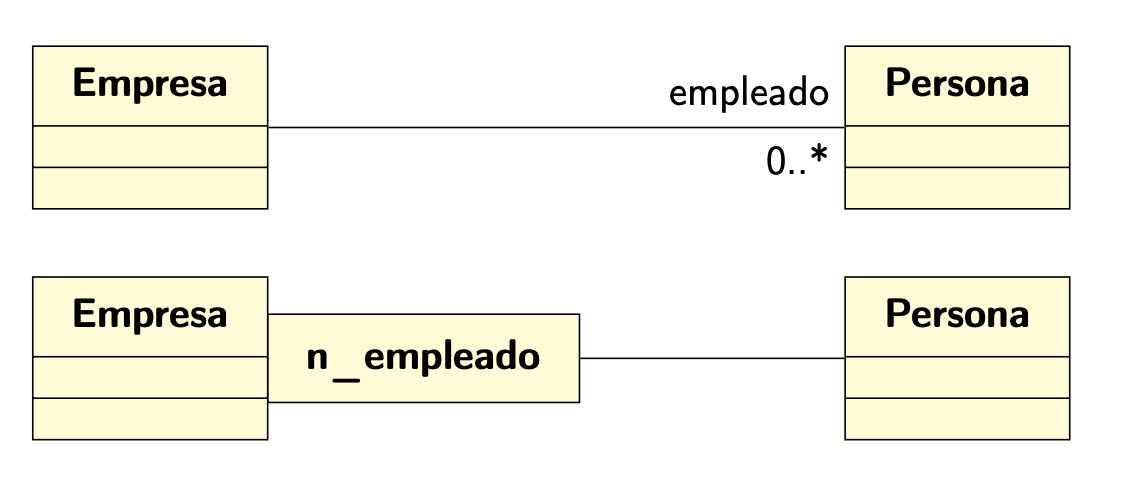
\includegraphics[width=\textwidth]{Imagenes/asc.png}\vspace*{0.2cm}
	\caption{Relaciones calificadas}
\end{figure}
Mediante esto, reducimos la multiplicidad en el lado muchos, haciendo las búsquedas mucho más eficientes.
Solamente podemos hacer uso de un atributo que sea \textit{clave primaria} de la clase.
Pasamos de 1 - muchos a 1 - 1.
Lo implementamos mediante un diccionario en la clase empresa.
Si la multiplicidad no se reduce, significa que dicho calificador no es \textbf{clave primaria} y por tanto, se pueden obtener diferentes valores para dicha clave.
\newpage
\subsection{Implementación de la relacion}
\begin{lstlisting}[frame=single]
class Empresa{
  public:
//mediante un calificador, encontramos un objeto de la clase Persona
    typedef std::map<C,Persona*>Bcalificada; 
    //métodos de la clase
    void asocia(Persona&);
    const Bcalificada& getA()const;
  private:
    Bcalificada bc_;
};
class Persona{
  public:
    //métodos propios de la clase
    typedef std::set<Empresa*>As;
    void asocia(Empresa&);
    const As& getB()const;
  private:
    C calificador; //calificador de tipo C
    As as_;
};
\end{lstlisting}